% Source-faithful topology: regular octagon, P on A6A7, vectors A1A3 and A1P.
% P is placed at a schematic interior point of the side; its exact position is not specified.
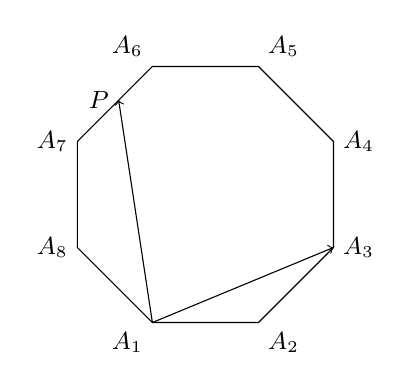
\begin{tikzpicture}[scale=0.88, every node/.style={font=\small}]
  \coordinate (A1) at ({2*cos(247.5)}, {2*sin(247.5)});
  \coordinate (A2) at ({2*cos(292.5)}, {2*sin(292.5)});
  \coordinate (A3) at ({2*cos(337.5)}, {2*sin(337.5)});
  \coordinate (A4) at ({2*cos(22.5)}, {2*sin(22.5)});
  \coordinate (A5) at ({2*cos(67.5)}, {2*sin(67.5)});
  \coordinate (A6) at ({2*cos(112.5)}, {2*sin(112.5)});
  \coordinate (A7) at ({2*cos(157.5)}, {2*sin(157.5)});
  \coordinate (A8) at ({2*cos(202.5)}, {2*sin(202.5)});
  \draw (A1) -- (A2) -- (A3) -- (A4) -- (A5) -- (A6) -- (A7) -- (A8) -- cycle;
  \path (A6) -- (A7) coordinate[pos=0.45] (P);
  \draw[->] (A1) -- (A3);
  \draw[->] (A1) -- (P);
  \node[below left] at (A1) {$A_1$};
  \node[below right] at (A2) {$A_2$};
  \node[right] at (A3) {$A_3$};
  \node[right] at (A4) {$A_4$};
  \node[above right] at (A5) {$A_5$};
  \node[above left] at (A6) {$A_6$};
  \node[left] at (A7) {$A_7$};
  \node[left] at (A8) {$A_8$};
  \node[left] at (P) {$P$};
\end{tikzpicture}
